%% REPLACE SXXXXXX with your student number
\def\studentNumber{S2890639}


%% START of YOUR ANSWERS
%% Add answers to the questions below, by replacing the text inside the brackets {} for \youranswer{ "Text to be replaced with your answer." }. 
%
% Do not delete the commands for adding figures and tables. Instead fill in the missing values with your experiment results, and replace the images with your own respective figures.
%
% You can generally delete the placeholder text, such as for example the text "Question Figure 2 - Replace the images ..." 
%
% There are 18 TEXT QUESTIONS (a few of the short first ones have their answers added to both the Introduction and the Abstract). Replace the text inside the brackets of the command \youranswer with your answer to the question.
%
% There are also 3 "questions" to replace some placeholder FIGURES with your own, and 3 "questions" asking you to fill in the missing entries in the TABLES provided. 
%
% NOTE! that questions are ordered by the order of appearance of their answers in the text, and not by the order you should tackle them. Specifically, you cannot answer Questions 2, 3, and 4 before concluding all of the relevant experiments and analysis. Similarly, you should fill in the TABLES and FIGURES before discussing the results presented there. 
%
% NOTE! If for some reason you do not manage to produce results for some FIGURES and TABLES, then you can get partial marks by discussing your expectations of the results in the relevant TEXT QUESTIONS (for example Question 8 makes use of Table 1 and Figure 2).
%
% Please refer to the coursework specification for more details.


%% - - - - - - - - - - - - TEXT QUESTIONS - - - - - - - - - - - - 



%% Question 1:
\newcommand{\questionOne} {
\youranswer{Early in training, training accuracy has a large positive velocity and training error a 
large negative velocity, indicating rapid fit. The validation curves show smaller magnitudes and their
 velocities decay toward zero as learning saturates. Around epoch 20, the validation accuracy velocity 
 crosses from positive to negative (the curve peaks), while the validation error velocity crosses from 
 negative to positive (the curve bottoms out). Meanwhile, training velocities remain favorable. This 
 divergence still improving while validation starts worsening indicates overfitting
}
}

%% Question 2:
\newcommand{\questionTwo} {
\youranswer{Question 2 - Present your network width experiment results by using the relevant figure and table||
the validation accuracy improves only marginally with increased network width—rising by 3\% from 32 to 64 
units and by 0.1\% from 64 to 128 units. Training curves show that wider networks converge faster and achieve 
lower training error, decreasing by 58\% and 53\% across these increments, respectively. However, the validation 
error increases by 38\% between 64 and 128 units, suggesting diminishing returns and potential overfitting at higher widths.
}
}

%% Question 3:
\newcommand{\questionThree} {
\youranswer{Question 3 - Discuss whether varying width affects the results in a consistent way, and whether the results are expected and match well with the prior knowledge (by which we mean your expectations as are formed from the relevant Theory and literature)
|| Increasing network width consistently improves training performance, as reflected by lower error and faster convergence. 
This aligns with theoretical expectations that wider networks have greater capacity to model complex functions. However, 
the minimal gains in validation accuracy and the rise in validation error at higher widths indicate overfitting, consistent
 with prior findings that overly large models can memorize training data without improving generalization. Overall, the 
 results align with theoretical predictions while illustrating the trade-off between model capacity and generalization.
}
}

%% Question 4:
\newcommand{\questionFour} {
\youranswer{Question 4 - Present your network depth experiment results by using the relevant figure and table ||
Validation accuracy improves modestly with increased network depth, rising by 0.8\% from 1 to 2 layers and by 0.1\% 
from 2 to 3 layers. Training curves show slightly faster convergence and lower training error, decreasing by 45\% 
and 5\% across these increments, respectively. However, validation error rises by 61\% between 1 and 2 layers and by 
9\% between 2 and 3 layers, suggesting diminishing returns and overfitting at higher depths. This trend is reflected 
in Figure~\ref{fig:depth_acccurves} and Figure~\ref{fig:depth_errorcurves}, where training performance continues to 
improve while validation performance plateaus and diverges after approximately 20 epochs.
}
}

%% Question 5:
\newcommand{\questionFive} {
\youranswer{Question 5 - Discuss whether varying depth affects the results in a consistent way, and whether the results are expected and match well with the prior knowledge (by which we mean your expectations as are formed from the relevant Theory and literature)
|| Increasing network depth yields consistent improvements in training performance, which aligns with theoretical 
expectations that deeper architectures can represent more complex mappings. However, the limited gains in validation 
accuracy and the rising validation error indicate overfitting, consistent with prior literature suggesting that deeper 
networks require additional regularization or data to generalize effectively. Overall, the observed results match 
expected theoretical trends, showing the balance between representational capacity and generalization.
}
}


%% Question 6:
\newcommand{\questionSix} {
\youranswer{Question 6 - Explain how one could use a combination of L1 and L2 regularisation. Discuss any potential benefits of this approach. Present an equation for this combined loss function and explain all relevant variables and hyperparameters.}
}


%% Question 7:
\newcommand{\questionSeven} {
\youranswer{Question 7 - Assume you had a limited experiment budget for exactly \textbf{4} experiment runs dedicated to testing the effectiveness of your proposed combination of L1 and L2 Regularization in Section~\ref{sec:L1L2combo}. Argue for which 4 configurations to run based on any previous results or other information you consider relevant. Run those experiments and add the results in Table~4 and Figure~5 (you will then discuss those results alongside all others in the next question below).

(Even if you have not managed to implement your L1 and L2 combination; still argue based on your proposed approach).

}
}


%% Question 8:
\newcommand{\questionEight} {
\youranswer{Question 8 - Explain the experimental details (e.g. hyperparameters), discuss the results in terms of their generalisation performance and overfitting. Select and test the best performing model as part of this analysis.
}
}


%% Question 9:
\newcommand{\questionNine} {
\youranswer{Question 9 - A colleague proposed using a custom activation function (which can be identified as CustomActivationLayer() in your Coursework\_1.ipynb notebook and the mlp package). Run the prepared experiment in the "Problematic Training" cell in your Coursework\_1.ipynb notebook, and display the results in Figure~6. Analyse the results. Is the model overfitting? Explain the cause of the problematic performance of the model?
}
}




%% Question 10:
\newcommand{\questionTen} {
\youranswer{Question 10 - Briefly draw your conclusions based on the results from the previous sections (what are the take-away messages?), discussing them in the context of the overall literature, and conclude your report with a recommendation for future directions}
}

%% - - - - - - - - - - - - FIGURES - - - - - - - - - - - - 

%% Question Figure 2:
\newcommand{\questionFigureTwo} {
\youranswer{Question Figure 2 - Replace the images in Figure 2 with figures depicting the accuracy and error, training and validation curves for your experiments varying the number of hidden units.
%
\begin{figure}[t]
    \centering
    \begin{subfigure}{\linewidth}
        
\includegraphics[width=\linewidth]{figures/mlp_cw1_emnist_hidden_units_comparison_accuracy.pdf}
        \caption{accuracy by epoch}
        \label{fig:width_acccurves}
    \end{subfigure} 
    \begin{subfigure}{\linewidth}
        \centering
        
\includegraphics[width=\linewidth]{figures/mlp_cw1_emnist_hidden_units_comparison_error.pdf}
        \caption{error by epoch}
        \label{fig:width_errorcurves}
    \end{subfigure} 
    \caption{Training and validation curves in terms of classification accuracy (a) and cross-entropy error (b) on the EMNIST dataset for different network widths.}
    \label{fig:width}
\end{figure} 
}
}

%% Question Figure 3:
\newcommand{\questionFigureThree} {
\youranswer{Question Figure 3 - Replace these images with figures depicting the accuracy and error, training and validation curves for your experiments varying the number of hidden layers.
%
\begin{figure}[t]
    \centering
    \begin{subfigure}{\linewidth}
        
\includegraphics[width=\linewidth]{figures/mlp_cw1_emnist_128_depth_comparison_accuracy.pdf}
        \caption{accuracy by epoch}
        \label{fig:depth_acccurves}
    \end{subfigure} 
    \begin{subfigure}{\linewidth}
        \centering
        
\includegraphics[width=\linewidth]{figures/mlp_cw1_emnist_128_depth_comparison_error.pdf}
        \caption{error by epoch}
        \label{fig:depth_errorcurves}
    \end{subfigure} 
    \caption{Training and validation curves in terms of classification accuracy (a) and cross-entropy error (b) on the EMNIST dataset for different network depths.}
    \label{fig:depth}
\end{figure} 
}
}

%% Question Figure 4:
\newcommand{\questionFigureFour} {
\youranswer{Question Figure 4 - Replace these images with figures depicting the Validation Accuracy and Generalisation Gap (difference between validation and training error) for each of the experiment results varying the Dropout inclusion rate, and L1/L2 weight penalty depicted in Table 3 (including any results you have filled in).
%
\begin{figure*}[t]
    \centering
    \begin{subfigure}{.475\linewidth}
        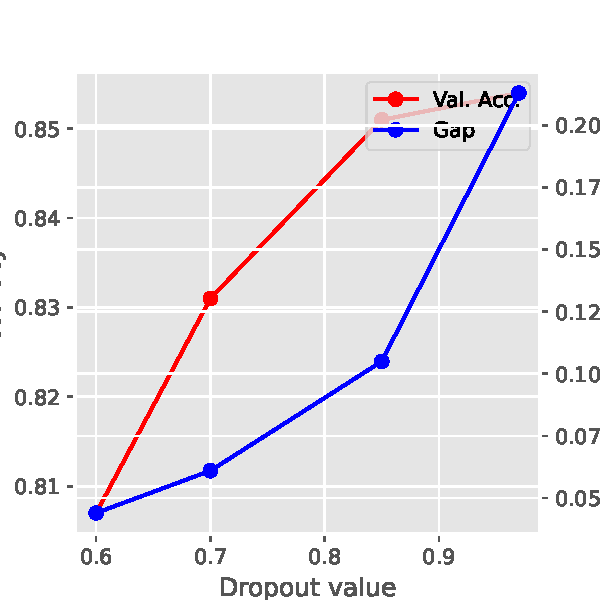
\includegraphics[width=\linewidth]{figures/mlp_cw1_emnist_dropout_accuracy_gap.pdf}
        \caption{Accuracy and error by inclusion probability.}
        \label{fig:dropoutrates}
    \end{subfigure} 
    \begin{subfigure}{.475\linewidth}
        \centering
        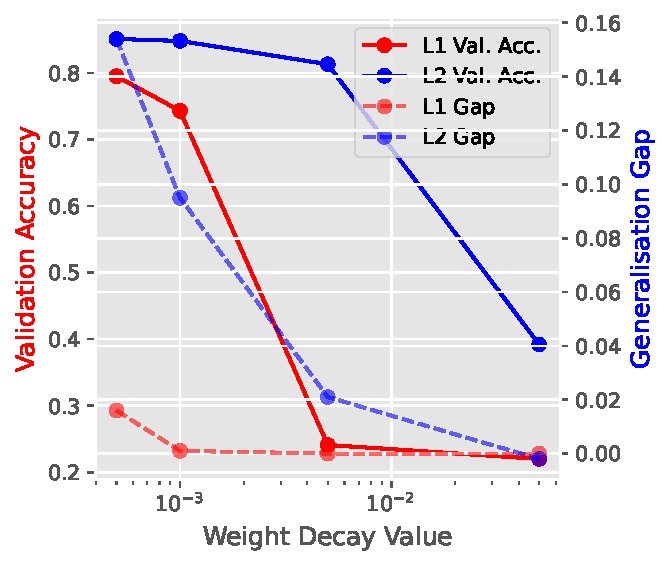
\includegraphics[width=\linewidth]{figures/mlp_cw1_emnist_weightdecay_accuracy_gap.pdf}
        \caption{Accuracy and error by weight penalty.}
        \label{fig:weightrates}
    \end{subfigure} 
    \caption{Accuracy and error by regularisation strength of each method (Dropout and L1/L2 Regularisation).}
    \label{fig:hp_search}
\end{figure*}
}
}

%% Question Figure 5:
\newcommand{\questionFigureFive} {
\youranswer{Question Figure 5 - Replace these images with figures depicting the Validation Accuracy, Training Accuracy, and Generalisation Gap (difference between validation and training performance) for each of the experiment results varying the Dropout inclusion rate and L1/L2 weight penalty depicted in Table 3 (including any results you have filled in).
%
\begin{figure*}[t]
    \centering
    \begin{subfigure}{.475\linewidth}
        
\includegraphics[width=\linewidth]{figures/mlp_cw1_emnist_l1l2_accuracy_gap.pdf}
        \caption{Validation and training accuracy, and generalisation gap for l1+l2 weight penalty.}
        \label{fig:dropoutrates}
    \end{subfigure} 
    \hfill
    \begin{subfigure}{.475\linewidth}
        \centering
        
\includegraphics[width=\linewidth]{figures/mlp_cw1_emnist_l1l2_error_gap.pdf}
        \caption{Training and validation error, and generalisation gap for l1+l2 weight penalty.}
        \label{fig:weightrates}
    \end{subfigure} 
    \caption{Training and validation performance across regularisation strengths for L1/L2 methods. The generalisation gap highlights overfitting effects across experiments.}
    \label{fig:hp_search}
\end{figure*}
}
}


%% Question Figure 6:
\newcommand{\questionFigureSix} {
\youranswer{Question Figure 6 - Add figures depicting the Training Accuracy, Error, and Gradient Flow Across Layers for the 1 experiment run with the Custom Activation function (produce these by running the "Problematic Training" cell in the Coursework\_1.ipynb notebook).
}
}

%% - - - - - - - - - - - - TABLES - - - - - - - - - - - - 

%% Question Table 1:
\newcommand{\questionTableOne} {
\youranswer{
Question Table 1 - Fill in Table 1 with the results from your experiments varying the number of hidden units.
%
\begin{table}[t]
    \centering
    \begin{tabular}{c|ccc}
    \toprule
        \# Hidden Units & Val. Acc. & Train Error & Val. Error\\
    \midrule
         32            &    78.8   &  0.558 &   0.691            \\
         64            &    81.00   &  0.353  &   0.665               \\
         128           &    81.1   &  0.165  &   0.918           \\ 
    \bottomrule
    \end{tabular}
    \caption{Validation accuracy (\%) and training/validation error (in terms of cross-entropy error) for varying network widths on the EMNIST dataset.}
    \label{tab:width_exp}
\end{table}
}
}

%% Question Table 2:
\newcommand{\questionTableTwo} {
\youranswer{
Question Table 2 - Fill in Table 2 with the results from your experiments varying the number of hidden layers.
%
\begin{table}[t]
    \centering
    \begin{tabular}{c|ccc}
    \toprule
        \# Hidden Layers & Val. Acc. & Train Error & Val. Error \\
    \midrule
         1               &      81.1      &   0.165 & 0.918                \\
         2               &      81.8      &   0.091 & 1.480                \\
         3               &      81.9      &   0.096 & 1.620                \\ 
    \bottomrule
    \end{tabular}
    \caption{Validation accuracy (\%) and training/validation error (in terms of cross-entropy error) for varying network depths on the EMNIST dataset.}
    \label{tab:depth_exps}
\end{table}
}
}

%% Question Table 3:
\newcommand{\questionTableThree} {
\youranswer{
Question Table 3 - Fill in Table 3 with the results from your experiments for the missing hyperparameter values for each of L1 regularisation, L2 regularisation, Dropout and label smoothing (use the values shown on the table).
%
\begin{table*}[t]
    \centering
    \begin{tabular}{c|c|ccc}
    \toprule
        Model    &  Hyperparameter value(s) & Validation accuracy & Train Error & Validation Error \\
    \midrule
    \midrule
        Baseline &  -                    &               83.7 &       0.241 &  0.533          \\
    \midrule
        \multirow{4}*{Dropout}
                 & 0.6                   &  80.7                &      0.549 & 0.593     \\
                 & 0.7 & 83.1 & 0.448 & 0.509  \\
                 & 0.85 & 85.1 &  0.329 &  0.434 \\
                 & 0.97 & \textbf{\emph{85.4}} &  \textbf{\emph{0.244}} & \textbf{\emph{0.457}}  \\
    \midrule
        \multirow{4}*{L1 penalty}
                 & 5e-4 & \emph{79.5} & \emph{0.642} & \emph{0.658} \\
                 & 1e-3 & 74.3 & 0.879 & 0.880 \\
                 & 5e-3 & 2.41 & 3.850 & 3.850 \\
                 & 5e-2 & 2.20 & 3.850 & 3.850 \\
    \midrule
        \multirow{4}*{L2 penalty}  
                 & 5e-4 & \emph{85.1} & \emph{0.306} & \emph{0.460} \\
                 & 1e-3 & 84.8 & 0.358 & 0.453 \\
                 & 5e-3 & 81.3 & 0.586 & 0.607 \\
                 & 5e-2 & 39.2 & 2.258 & 2.256  \\
    \midrule
        Label smoothing & 0.1 & 84.9 & 1.02 & 1.16 \\
    \bottomrule
    \end{tabular}
    \caption{Results of all hyperparameter search experiments. \emph{italics} indicate the best results per series (Dropout, L1 Regularisation, L2 Regularisation, Label smoothing) and \textbf{bold} indicates the best overall.}
    \label{tab:hp_search}
\end{table*}
}
}


%% Question Table 4:
\newcommand{\questionTableFour} {
\youranswer{
Question Table 4 - Results from 4 training runs varying L1+L2 regularisation.
%
\begin{table*}[t]
    \centering
    \begin{tabular}{c|c|ccc}
    \toprule
        Run & L1 / L2 & Val. Acc. (\%) & Train Error & Val. Error \\
    \midrule
         1 & $1\times10^{-6}$ / $1\times10^{-4}$ & 84.6 & 0.252 & 0.486 \\
         2 & $1\times10^{-5}$ / $1\times10^{-4}$ & 84.7 & 0.268 & 0.469 \\
         3 & $1\times10^{-6}$ / $5\times10^{-5}$ & 84.0 & 0.250 & 0.507 \\
         4 & $1\times10^{-5}$ / $5\times10^{-5}$ & 84.3 & 0.267 & 0.488 \\
    \bottomrule
    \end{tabular}
    \caption{Validation accuracy (\%) and training/validation cross-entropy error for four runs with different L1/L2 hyperparameters (L1 / L2 shown in a single column to match the size/format of Table~3).}
    \label{tab:l1l2_exps}
\end{table*}
}
}

%% END of YOUR ANSWERS